\section{Linemod template matching} \label{sec:linemod}
Template matching has always been an attractive approach to computer vision,
especially for real-time applications; some of the main reasons for this
include ease of generalization of
these algorithms (several shapes can be associated to the same object), and
variety of applications (from rigid object detection -- like in this project --
to face recognition); another great advantage over other recognition methods,
such as neural networks, is the need of a relatively simple and fast training phase:
statistics-based methods, in turn, usually require a huge amount 
of samples to be given for evaluation. Usage of template matching also opens
the possibility of starting with a small, offline-generated template database, and training the
objects to be recognized \emph{online}, i.e. acquiring new samples while
recognizing them. In this sense, template matching offers both the benefits of
a fast, model-based training stage and the benefits deriving from
machine-learning algorithms, improving their performance the more they operate.

Two usual problems often come with template-based solutions: the first is that,
as a template usually consists of a set of features to be searched into the
target image, the high-number of templates (even for a relatively small
database) makes this technique come with an extremely high computational cost;
on the other hand, statistical methods require a much longer training phase but
usually base themselves, at recognition time, on a well-defined, very small set of
data (e.g. hue histograms, network coefficients) which is not proportional to the number of elements
analyzed during training phase. Also, template matching usually has poor
results when the analyzed object has little texturing information, as a low
number of features (\emph{keypoints}) can be extracted for each datum.

The Line-MOD template matching algorithm was introduced in 2011 by
Hintestoi{\ss}er, S. et al. (\cite{linemod-paper}) as a way to address these
two problems of template matching approaches. It is based on a previous work by
the same authors, \cite{linemod-origins}, in which the LINE algorithm was
descripted, which solved both the problem of template matching velocity and
texture-less detection, modified to give increased robustness and detection
rates. Another, following work is described in details in sec.
\ref{sec:linemod-pipeline}, and focuses on a practical application of these
algorithms, which is the one to which the system proposed into this project has
inspired.

In this section, this algorithm is explained in detail. Its key concepts are
introduced first, such the concept of image gradient (sec.
\ref{sec:linemod-gradient}) and depth normal computation (sec.
\ref{sec:linemod-depth}). Then, the modality of data representation, which is
the main reason for this algorithm's good performance, is shown in sec.
\ref{sec:linemod-binary}, and finally the algorithm's operating principle is
detailed in sec. \ref{sec:linemod-usage}.

\subsection{Gradient orientation of images} \label{sec:linemod-gradient}
In order to efficiently detect matches into a non-textured image, which is one
of the problems which Line-MOD proposes to solve, a good metric that can be
used for defining salient features into the image is the value (and direction)
of the image \emph{gradient} $\vec{\nabla} (u,v)$ for each pixel. This vector
quantity is defined just like the discrete gradient for a function on the
domain $N$ of natural numbers: by quantizing the differential operator, the
discrete derivate of a function $f(x)$ is given by

\begin{equation}
\frac{df(x)}{dx}=f(x+1)-f(x)
\end{equation}

At the same way, an image can be seen as a set of  functions (one for each
channel) of two variables $(u,v)$, returning the corresponding pixel value at
the desired coordinate, for the desired channel. Thus, a partial, discrete
derivative can be computed onto this function, and the gradient can be defined
as usual as the vector of partial derivatives:

\begin{eqnarray}
\frac{\partial f(u,v)}{\partial u} & = & f(u+1,v)-f(u,v) \\
\frac{\partial f(u,v)}{\partial v} & = & f(u,v+1)-f(u,v) \\
\nabla f(u,v) = \begin{pmatrix} \frac{\partial f(u,v)}{\partial u} \\
\frac{\partial f(u,v)}{\partial v} \end{pmatrix} & = &
\begin{pmatrix}f(u+1,v)\\ f(u,v+1)\end{pmatrix}-\begin{pmatrix}f(u,v) \\
f(u,v)\end{pmatrix}
\end{eqnarray}

This is, anyway, an informal definition, which neverthless finds its
application being simple to implement and computationally cheap. More formal
definitions exist, such the \emph{Sobel operator}, which instead of scanning the
image for difference into a single direction linearly approximates the image as
a continuous function -- it assumes, in fact, that the underlying intensity
function for each channel is continuous
and sampled only in correspondance of pixels' coordinates -- , and thus makes
uses of a convolution operator to approximate samples of the continuous
gradient $G(f)$:

\begin{eqnarray}
  G_x(f) &=& \begin{pmatrix} 
      -1 & 0 & 1 \\
      -2 & 0 & 2 \\
      -1 & 0 & 1 \end{pmatrix}
  \ast f \\
  G\_y(f) &=& \begin{pmatrix} 
      -1 & -2 & -1 \\
      0 & 0 & 0 \\
      1 & 2 & 1 \end{pmatrix}
  \ast f  \\
  G(f) & = & \begin{pmatrix} G_x \\ G_y \end{pmatrix}
\end{eqnarray}

Here, the $\ast$ operator represents convolution of a $3\times 3$ matrix $K$, called
\emph{kernel}, with another matrix $A$: after extending $A$ with a row of $0$ on
each of its four sides, the value of $K\ast A$ is defined for each coordinate
$(u,v)$ as:
\begin{equation}
  (K \ast A)_{u,v} = \text{sum}\begin{pmatrix}
    K_{0,0}A_{u-1,v-1} & 
    K_{0,1}A_{u,v-1} & 
    K_{0,2}A_{u+1,v-1} \\ 
    K_{1,0}A_{u-1,v} & 
    K_{1,1}A_{u,v} & 
    K_{1,2}A_{u+1,v} \\ 
    K_{2,0}A_{u-1,v+1} & 
    K_{2,1}A_{u,v+1} & 
    K_{2,2}A_{u+1,v+1}  
  \end{pmatrix}
\end{equation}

Depending on how the gradient of the image is approximated, the result could
slightly change. However, the intuitive concept is always the same. As an
example, the result of the application of Sobel operator $G$ on a reference
image\footnote{Image taken from the USC SIPI database
  ( http://sipi.usc.edu/database/ ), one of the most common computer vision reference
databases. Original source is unknown.}
 is shown in fig.\ref{fig:scimmia}.

\begin{figure}[htbp]
\centering
\begin{tabular}{c|c}
  \multicolumn{2}{c}{\adjustbox{valign=m}{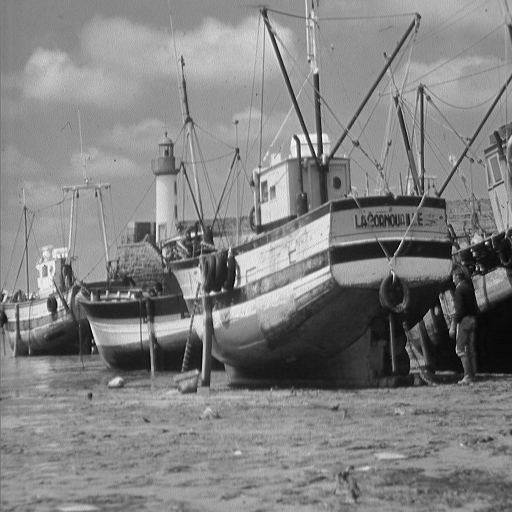
\includegraphics[height=2in]{./Graphics/scimmia}}} \\
    \multicolumn{2}{c}{\vspace{0.2in}} \\
  \adjustbox{valign=m}{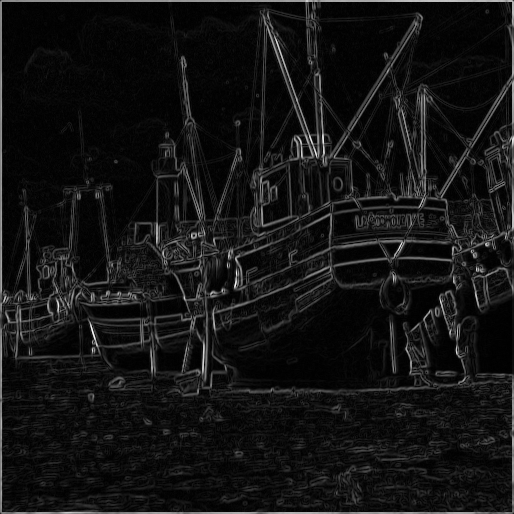
\includegraphics[height=2in]{./Graphics/scimmiagradient}} &
  \adjustbox{valign=m}{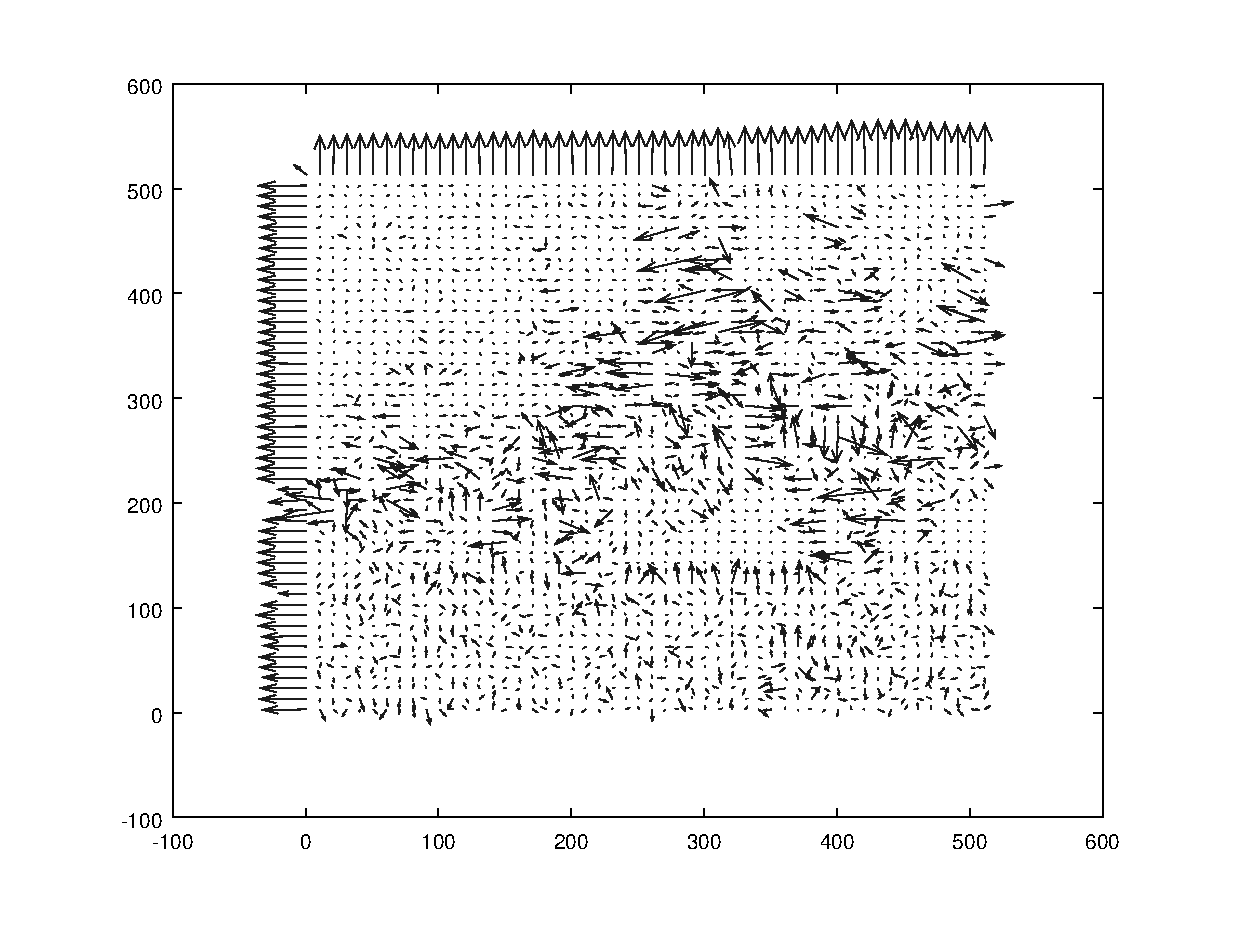
\includegraphics[height=2.5in]{./Graphics/scimmiafrecce}}
\end{tabular}
\caption{Grayscale, single-channel image (top) on which the Sobel operator $G$
has been applied. Resulting absolute value (left) and vector field
(right).\label{fig:scimmia}}
\end{figure}

\subsection{Fast normal computation from depth images} \label{sec:linemod-depth}
One of the most important features which can be extracted from a 3D
image is points' normals. These, just like an image's gradient, form a
vector field inside the image, representing the approximated normals
to the surface for which the RGBD picture has been taken, sampled in
correspondance of the image's pixel centers.

Of course, starting with sampled (and noisy) data from the image
implies that the normals which are computed are only a supposition:
if it is assumed that the quantized depth value is sufficient to give
informations about normals, the assumption must also be made that the
function is almost flat in local neighbourhoods, otherwise the Nyquist
theorem would be violated. With this assumption, neverthless, it is
possible to approximate the planar surface corresponding to each pixel
with a plane connecting the plane and each of its neighbour points,
and from this compute the normal vector to each point.

The Line-MOD algorithm in its original implementation
(\cite{linemod-paper}) makes use of this idea to compute normals which will be used
as a feature for templates.

First, for each point $p$ in the image, the neighbour pixels are
considered. Assuming that the objects to be computed could be into a
cluttered scene, however, before taking each of them, a check is done
for drastic changes in the depth value $d$: if the variation is too
high (over a certain threshold $t_d$), this means that two separate
surface are actually considered, and this would break the assumptions
stated before, so the pixel is discarded; this technique also removes
possible outliers caused by bad sensor's performance.  The remaining pixels are put
into a neighbourhood set $N_p$. 

Considering the hypotetical plane which $p$ belongs to, its
orientation can be described by means of the gradient $\nabla$ of the
depth function $D(u,v)$. This, in turn, can be approximated by using first-order
Taylor expansion over the $(u,v)$ coordinate. For every point $p_2 \in N_p$:

\begin{eqnarray}
  p_2 & = & \begin{pmatrix} u_2 \\ v_2 
  \end{pmatrix} \\
  D(p_2)-D(p) & = & dp^{\tau}\nabla D (p) + o (p) \text{(taylor
    expansion)} \label{eqn:taylor-depth-expansion}\\
  \nabla d(u,v) \approx \begin{pmatrix} \frac{\partial d(u,v)}{\partial u}
    \\ \frac{\partial d(u,v)}{\partial v}
  \end{pmatrix} & = & \begin{pmatrix} \frac{d(u2,v2)-d(u,v)}{u2-u} \\
    \frac{d(u2,v2)-d(u,v)}{v2-v} 
  \end{pmatrix}
\end{eqnarray}

With this approximation, each of the points in $N_p$ defines a
constraint over $N_p$, which is defined with the reasonable assumption
that at least 2 points in the neighbourhood will be considered
(otherwise, a null normal vector will be assigned to $p$). In the best
case of 8 valid neighbours, each of them is considered and, being the
system over-constrained, the
gradient $\nabla$ is computed in order to minimize the least-squared
error on eqn.\ref{eqn:taylor-depth-expansion}. This will smooth away
the noise on depth due to sensor's limitations and values'
quantization (assuming it is randomly distributed).

After computing the best approximation for the depth function's
gradient over $p$, the normal vector $N(p)$ can be approximated by computing
two principal axes of the surface's plane and deriving it from the
external product of these two:

\begin{eqnarray}
  dU & = & D(p)+\frac{\partial D(p)}{\partial u} \\
  dV & = & D(p)+\frac{\partial D(p)}{\partial v} \\
  N(p) & = & \frac{dU \times dV}{\lVert dU \times dV \rVert}
\end{eqnarray}
This algorithm, which is similar to what is implemented by most 3D
processing libraries -- most notably, Point Cloud Library --, produces
a good result in terms of an acceptable precision and a very good
performance. In this case, the latter is much more important as
precision in normal computation will be not very relevant, as the
algorithm will highly cut down the resolution of this computation to
better stand small transformations as explained in
sec. \ref{sec:linemod-quantization}. On the other hand, computational speed
is important as Line-MOD wants to be able to have future real-time applications.

\subsection{Gradient and depth quantization} \label{sec:linemod-quantization}
The main innovation introduced by \cite{linemod-origins}, and thus by
\cite{linemod-paper}, is a big improvement over matching time due to
a novel, binary representation for templates' data. This
representation provides both fast matching time and robustness to small
deformation of the objects (or pose changes with respect to the
template's ground pose), as it spreads every feature into its surronding
area, thus making it possible to detect them even in the case in which
they perform a relative movement between each other.

Before coding each template data with a binary pattern, it is
\emph{quantized}. The number of quantization steps to be considered
will affect many aspects of the algorithm's behaviour; in particular,
an high number of steps will result in bigger templates, longer
execution time, but much fewer false positives, as more accuracy will
be needed for the features to match; for the same reason, it also will
decrease the algorithm's tolerance to illumination or camera
changes. On the other hand, a lower number of steps will imply more
tolerant matches: this will provide faster execution time and an
improved detection capability in case of template changes, but at the
cost of a high number of false positives, which will have to be filtered.

The Line algorithm of \cite{linemod-origins} only considered colour gradient; however, Line-MOD
generalized this algorithm to be capable to match different set of
features, each represented by a \emph{modality} comprehensive of a
feature-computation algorithm, a discretization one, and a match score
computation. In this way, the binary encoding and matching algorithms
can be applied to whatever feature set is more appropriate for the
template, and thus the whole algorithm can be easily extended and find
new application areas. In practice, in this implementation two
modalities have been used, which are colour gradient as described in
sec.~\ref{sec:linemod-gradient} and depth normals as in
sec.~\ref{sec:linemod-depth}, for which good computation algorithms have
been already stated.

Before discretization, every feature is discarded if it is not strong
enough, i.e. if its corresponding vector's magnitue is less that a
threshold $t_{filter}$. This helps too keep only the most important
features into the image, which is important as the feature's magnitude
will be flattened in the following steps.

For the image colour gradient, discretization of the gradient's direction is
considered; this is represented by the angle $\alpha$ from the
base of the positive $X$ axis to the gradient's direction line. Given
the number $N$ of samples, the orientation angle is approximated to
the nearest discrete quantity $\alpha_d = \frac{k\pi}{N}, k \in
{0\dots N-1}$. 
This process is repeated for each of the three (in case of an RGB
image) channels, and only the gradient with the strongest absolute
magnitude is kept. The result of this last step is a gradient which is
much more descriptive of the actual image, with respect to the
standardized technique of computing the gradient over the
corresponding greyscale image: as it can be seen from
fig. \ref{fig:duck-gradient}, in which the gradient has been computed
over a duck-toy image using both this and the standard algorithms,
borders are neatly identified: this approach is thus more appropriate for
template creation and detection. In this case the red arrow,
representing the gradient of a pixel into the image, is approximated
to the nearest location; also, as only the direction is considered,
the vector will never be approximated to a point lying into the lower
part of the angles' space.

\begin{figure}[htbp]
\centering
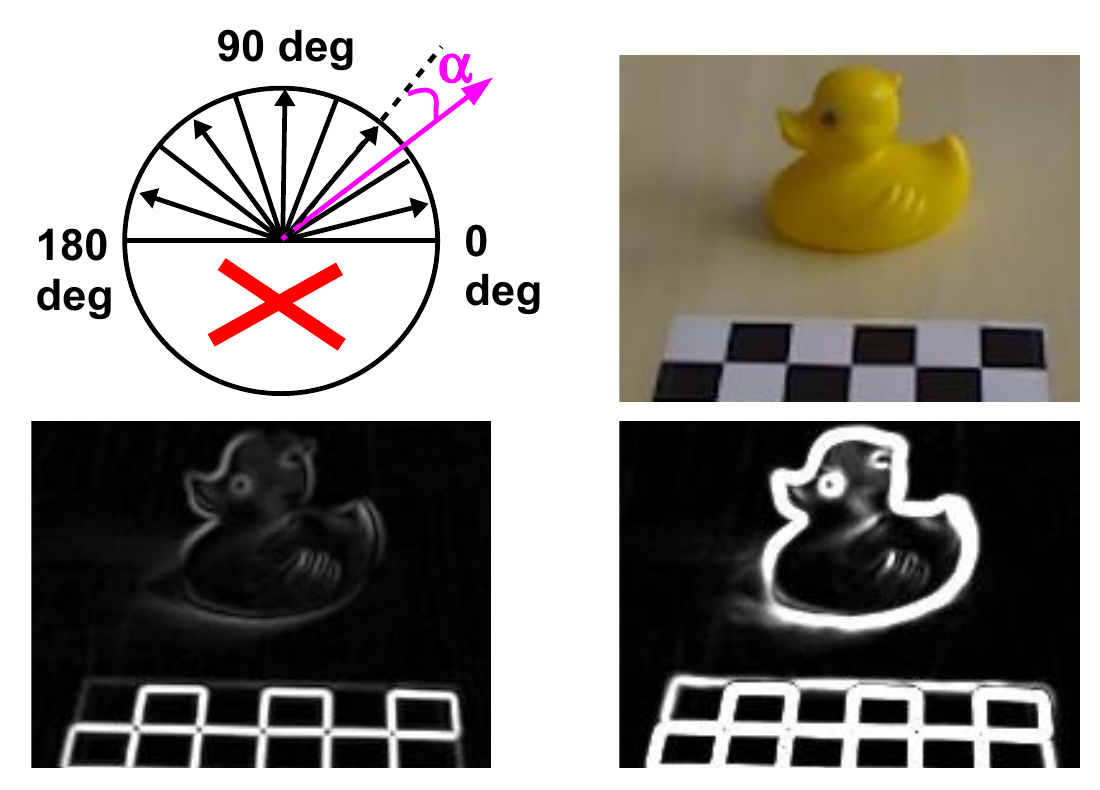
\includegraphics[height=2.5in]{./Graphics/duck-gradient}
\caption{Approximation of the gradient for the image of a duck toy:
  the discretization algorithm used by Line-MOD (right) provides a
  much better edge recognition performance with respect to standard
  algorithms (left). Image courtesy of Stefan Hinterstoi\ss er. \label{fig:duck-gradient}}.
\end{figure}

By considering only the direction of the gradient, and not its
full vector, two problems are solved: first, the gradient extracted
from the template will be compatible with the matching one,
independently of illumination changes. Second, by not taking into
account the way of the gradient, it will be valid both if the shape
stands on a dark background, and if it stands on a clear background:
the gradient will, in this case, mantain its module and direction and
only change its way, which will be discarded.

Regarding normals' discretization, the same considerations can be
applied. Dropping the normal vector's magnitude comes naturally, as
it will be $1$ by definition. Thus, again only the direction of the vector is
considered. Being a 3D vector, opposed to the 2D vector which is the
image's gradient, it is more difficult to find a good discretization
for the possible value. The solution of \cite{linemod-paper} is to
discretize the normals' direction with respect to a set of possible
directions over the edges of a right, circular cone pointing towards
the camera. Each vector is then first flattened to the edge of the
cone, then to the nearest sample: in this way, the obtained value
is a representation of the radial direction in which the normal is deviating from the
camera's axis, which is a reasonable definition for what the normals
conceptually mean. Also, using a cone as a reference surface allows to
have a higher approximation level with a lower number of discrete
quantities, as each vector spawning the same radial direction
(longitude) will be well-represented no matter its latitude.

As depth sensors suffer from measurement noise, especially on the high
distances, after computing each pixel's normal vector and assigning a
quantized value to it, a convolutionary filter is applied to the whole
image: for each pixel, the local $5\times 5$ neighbourhood is
considered, and to that pixel is assigned, as a final depth value, the
sample that occours most frequently into it (nulled normal vectors are
not considered at this step). This is useful as,
considering the surfaces as mostly smooth over a small area (sudden
changes in depth have been already removed by the normals' computation
step of sec.~\ref{sec:linemod-depth}), a voting algorithm can further
help with outliers' removal.

The result of this process can be seen in fig.~\ref{fig:depth-man}:
the man figured into the top-left corner has been captured with a
depth camera, and the resulting depth function can be seen in the
bottom-left corner; applying this quantization algorithm to the depth
map returns a result which is perfectly capable of distinguishing
different objects' borders (on which the image has been cut) and at
the same time subdivide smooth areas between each other.

\begin{figure}[htbp]
\centering
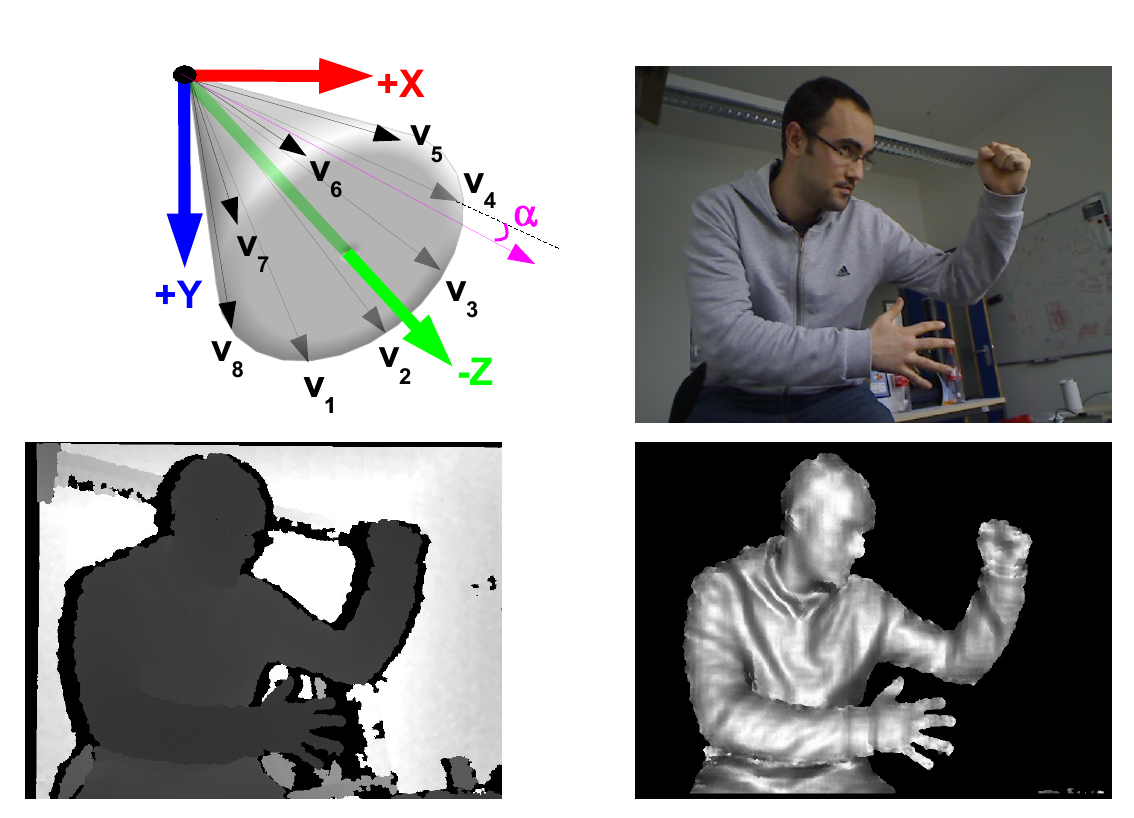
\includegraphics[height=2.5in]{./Graphics/depth-man}
\caption{Discretization of the possible values for a surface's normal
  vector to the surface of a circular cone (top-left). If applied to a
  real image (top-right), the input depth map (bottom-left) produces a
  normal map (bottom-right) which is already aware of difference
  between objects and can reproduce a good level of detail with
  respect to the original scene. Image courtesy of Stefan Hinterstoi\ss er. \label{fig:depth-man}}.
\end{figure}

\subsection{Binary representation of quantized images} \label{sec:linemod-binary}
After the images have been quantized, they are ready to be encoded
with a binary format, which is suitable for fast template
matching. Each quantized feature, being it gradient orientation,
normal orientation, or a custom one, is assigned to a $N$-bit value
($N$ representing the number of quantization levels), corresponding to
the value having a $1$ into one of its bits and $0$ into the other
ones: this allows a unique representation of both single values and
set of values. After this,
the values are ``spreaded'' in the neighbourhood of their corresponding
pixel. In simple term, each binary pixel from the previous step is
transformed into a binary pixel containing informations about which of
the quantization levels are present into the neighbourhood of size
$T$. At binary level, this is very easy and efficient to implement
given how the values are represented: in fact, it is sufficient to
generate $T^2$ images, each one shifted of a different number of
pixels in the range $\delta p = \left\{\left[-\frac{T}{2},
  \frac{T}{2}\right], \left[-\frac{T}{2},
  \frac{T}{2}\right]\right\}$; the result of a general \texttt{OR}
operation between all of these images will have the required
characteristics, as it will be formed of pixels having $1$ in the bits
corresponding to the features' values which are present at least once in
the adjacent pixels.

Spreading pixels in this way has the advantage of introducing at no
cost a good flexibility and robustness in terms of rigid deformation:
in fact, it mantains locality of features, but at the same time
permits to match features with a good margin of skew: the value of $T$
can be reduced if the algorithm is thought to be too permissive, but
it should never be deleted as this would cause all features to be
fixed to their pixel, which would cause obvious problems -- at least
due to the quantization error of the camera in terms of $(u,v)$
coordinates.

When the most important features have been spreaded in their surronding
area, non-null pixels are left; this is the final result of the
template creation process, and the corresponding template can be
stored in memory for future usage. It is important to notice that a
template is actually a \emph{collection} of these sets of pixels
(i.e. features): for an image $I$, the corresponding template built
from modality set $M$ is thus a set of sets, $T(I) = \left\{ S_m(I), m \in M \right\}$.

\subsection{Line-MOD runtime algorithm} \label{sec:linemod-usage}
With all the premises of the previous sections, the Line-MOD algorithm
can be described. Line-MOD is a subset of Line
(\cite{linemod-origins}), which takes the same processing steps of
Line and applies it to match multiple features, computed from
different modalities, in parallel (hence the name, for
\emph{multiple-MODalities Line}). After computing and discretizing
set of modalities, seen by the algorithm through a simple abstraction
layer given by these three operations (the process at the upper level
is thus, indeed, completely modality-agnostic), this algorithm
converts them to binary form and spreads them, as explained in
sec.~\ref{sec:linemod-binary}. Each binary image is at this point filtered
through a certain logic, given by the feature itself: for example,
considering the case of untextured objects, colour gradients can be
found mostly onto the external edges of the objects: thus, only these
are extracted after gradient computation, as this will improve a lot
the algorithm's performance without impacting the recognition process. %TODO esperimentino
On the other hand, considering normals on the edges would for sure
worsen the performance in terms of recognition accuracy, as normals
are not well-defined in proximity of the borders. Thus, normals are
filtered out and only those strictly inside the object are
considered. As shown in fig.~\ref{fig:duck-linemod}, this
complementary set of features, which cover the entire object if summed
up, is the main reason of the good performance of this algorithm with
respect to its predecessor as demonstrated in \cite{linemod-paper}.

\begin{figure}[htbp]
\centering
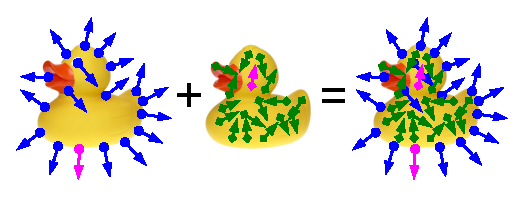
\includegraphics[width=4in]{./Graphics/duck-linemod}
\caption{Combination of different modalities, which is the main
  characteristic of the Line-MOD algorithm, allows to spread uniformly
  the detection of features upon the whole object, which is the main
  reason for its robustness. Image courtesy of Stefan Hinterstoi\ss er. \label{fig:duck-linemod}}.
\end{figure}

After feature spreading, each newly-created template is ready for
matching into an image. The scenario is thus changed from template
building to template matching, and the task to perform, for each
template $T$ which is put into a template list to be matched, is to
find a similarity measure $\epsilon_m (T,I)$ between the template itself
and a portion $P(I,c)$ of
the input image $I$, centered on $c$, on which the template has to be matched. Given a
similarity function $S_m(p_1, p_2)$ between two points $p_1$ and $p_2$
with respect to their discretized value with modality $m$ -- the ones
of which the templates' images are built -- the maximum similarity
score for each point in $P$ with respect to the corresponding
neighbour pixels in $T$ with maximum distance $r$ is taken, and these values are summed up:

\begin{equation} \label{eqn:similarity-function}
  \epsilon_m (T,I,c)=\sum_{p\in P(I,c)} { \left( \max \left\{ S_m
      (p,p_2) , p_2 \in P(c\dots c+r) \right\} \right) }
\end{equation}

Althought similarity functions can be customized, the main ones used
by the Line-MOD algorithm consider the difference of direction between
corresponding pixels:

\begin{eqnarray}
  S(I,T,p_1,p_2) & = & \lvert \cos(\text{ori}(I,p_1) -
  \text{ori}(T,p_2)) \rvert \text{(for gradient)} \\
  S(I,T,p_1,p_2) & = & \lvert N(I,p_1)^{\tau} N(T,p_2)\rvert \text{(for normals)}
\end{eqnarray}

Here, $\text{ori}(I,p)$ indicates the orientation of the strongest
gradient of I at point p, as computed in
sec.~\ref{sec:linemod-gradient}, while $N(I,p)$ indicates the
approximation of the normalized vector normal to the surface of I as
computed in sec.~\ref{sec:linemod-depth}.

This is a good conceptual algorithm, but it would be enormously slow
if applied ad-litteram for each template and point into the image, as
it would require score computation for each point into the template,
each point into the image, each point into the neighbourhood; this
would lead to a cost of $O(\text{size}(I)\times \text{size(T)}\times
r^2)$, which is obviously unacceptable. A new data structure is used for
the purpose of matching, which is described below; usage of this
structure can lower drastically the computation time and bring it back
again to good levels.

The basic consideration for this is that the actual number $n_0$ of levels (bins)
on which each feature will be quantized, and thus the possible values
to which each pixel in the image will be matched, is actually really low; if,
for example, 8 bins are used to quantize values, after spreading the
binary representation of each pixel will be 8 bits, and thus contain
64 possible values. It is thus perfectly feasible to do a one-shot,
a-priori computation of the score function $S$ for each possible
combination of input values. The spreaded image $I$ can be, in this way,
tranformed into another serie of images $\tau_i(I), i \in 1 \dots 2^{n_0}$, resorting a lookup table, in
which each pixel corresponds to a list of values for $S$ which can be
easily matched with each possible value into the template $T$ by only
indexing it. Once this lookup tables has been built, the total
similarity function $S(I,T,c)$ will thus be much more easier to compute:

\begin{equation}
  \epsilon_m (T,I,c)=\sum_{p\in P(I,c)} { \tau_{I[p]} }
\end{equation}

It should be noticed that the lookup tables $\tau_i$ must be computed
only once, which reduces the computational effort of the matching
algorithm.

The result of this implementation is a fast (the computationally
intensive part has been reduced to direct memory accesses) and
versatile (the modalities can be of any type, as long as they provide
the characterising functions) matching algorithm, which can associate
to each couple $(T_i,p_j)$ of possible positions of a template into
the input image an output value which is a good representation of how
much the template fits well the chosen part of input. A natural but
important consequence of this is that no template will be flagged as
matching or not by the algorithm itself, so for example in case of light objects'
occlusions the ``good'' matches will find themselves to be the
ones with the highest score no matter the situation. After doing
this, it sufficient to discard every match for which the matching
score is below a chosen threshold -- which can be adapted with the
tradeoff of recognition capabilities versus potential false positives,
but will have no impact over performance -- in order to correctly
detect objects in every scene. With the same steps it is possible to
match more than one object type at the time, by simply putting more
than one template set into the list of templates to be recognized, and
assign to each a label indicating the object's type.

\subsection{Memory linearization for fast memory access on modern
  CPUs}
Being, for certain aspects, a quite low-level kind of algorithm, and
exploiting binary logic operations and intensive lookup tables access
for its matches, Line-MOD can improve a lot its performance by
exploiting the hardware features available to modern processors. In
particular, if the lookup table is not accessed properly, a high
number (near $100\unit{\%}$) of cache misses will impact heavily onto
the algorithm's performance. Line-MOD introduces thus the concept of
\emph{memory linearization} (from which the name \emph{Line} comes) to
ensure that, at matching time, the best possible sequence of pixels
will be matched in order to minimize cache misses.

One of the advantages of spreading the features' values as done in
sec.~\ref{sec:linemod-binary} is the fact that, if a feature is
present at point $p(u,v)$, it will be present also in all of its
neighbourhood of size $t$. As the similarity function only considers the maximum
value for each point into the considered pixel, it will be sufficient
to match one each $t$ pixels: if the point $p$ would affect this
maximum value, it will actually affect it being in a neighbourhood; if
it wouldn't, it can safely be ignored as it value would be obscured by
the maximum pixel's value.

Checking one every $t$ pixels would of course reduce the number of
steps by a factor $t^2$, but it would cause a lot of problems with
memory cache as stated above. Thus, the lookup table $S_i(I)$ is
reorganized in memory before matching by taking each $t$-th
pixel (i.e. creating a subsampled image starting at $p$) and storing it in a contiguous memory region, in a row-major
way; this will cause most of the image's salient points to fit the L1
cache of the CPU. When the subsampled image ends, the same process is
reiterated starting from the position following $p$. At the end of the
process, the whole image will be represented in memory in a manner
which is similar to how interlaced formats work, as shown in fig.~\ref{fig:linemod-linearize}.

\begin{figure}[htbp]
\centering
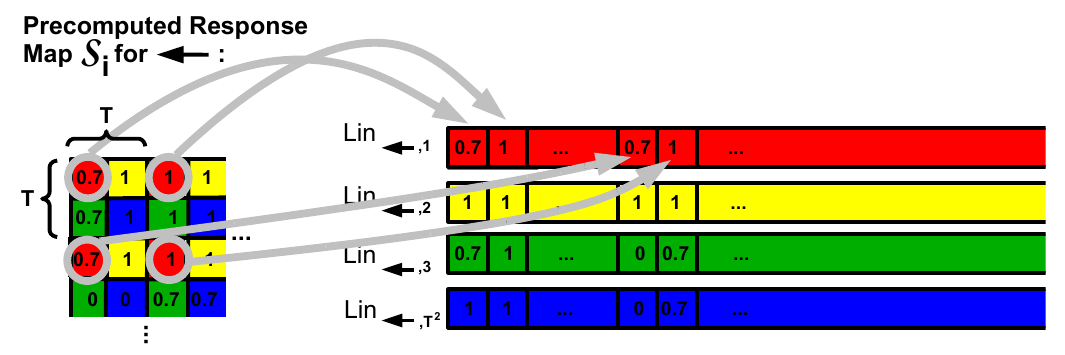
\includegraphics[width=5in]{./Graphics/linemod-linearize}
\caption{A precomputed lookup table $S_i(I)$ is, before matching,
  reorganized in memory so that the matching algorithm, taking one
  pixel every $t$, will seldom cause a cache miss. Image courtesy of Stefan Hinterstoi\ss er.\label{fig:linemod-linearize}}.
\end{figure}
